\begin{figure}[t]%
  \captionsetup[subfloat]{justification=RaggedLeft,singlelinecheck=false}
    \centering
    \subfloat[\\Band-doubling\\(\edlib)]{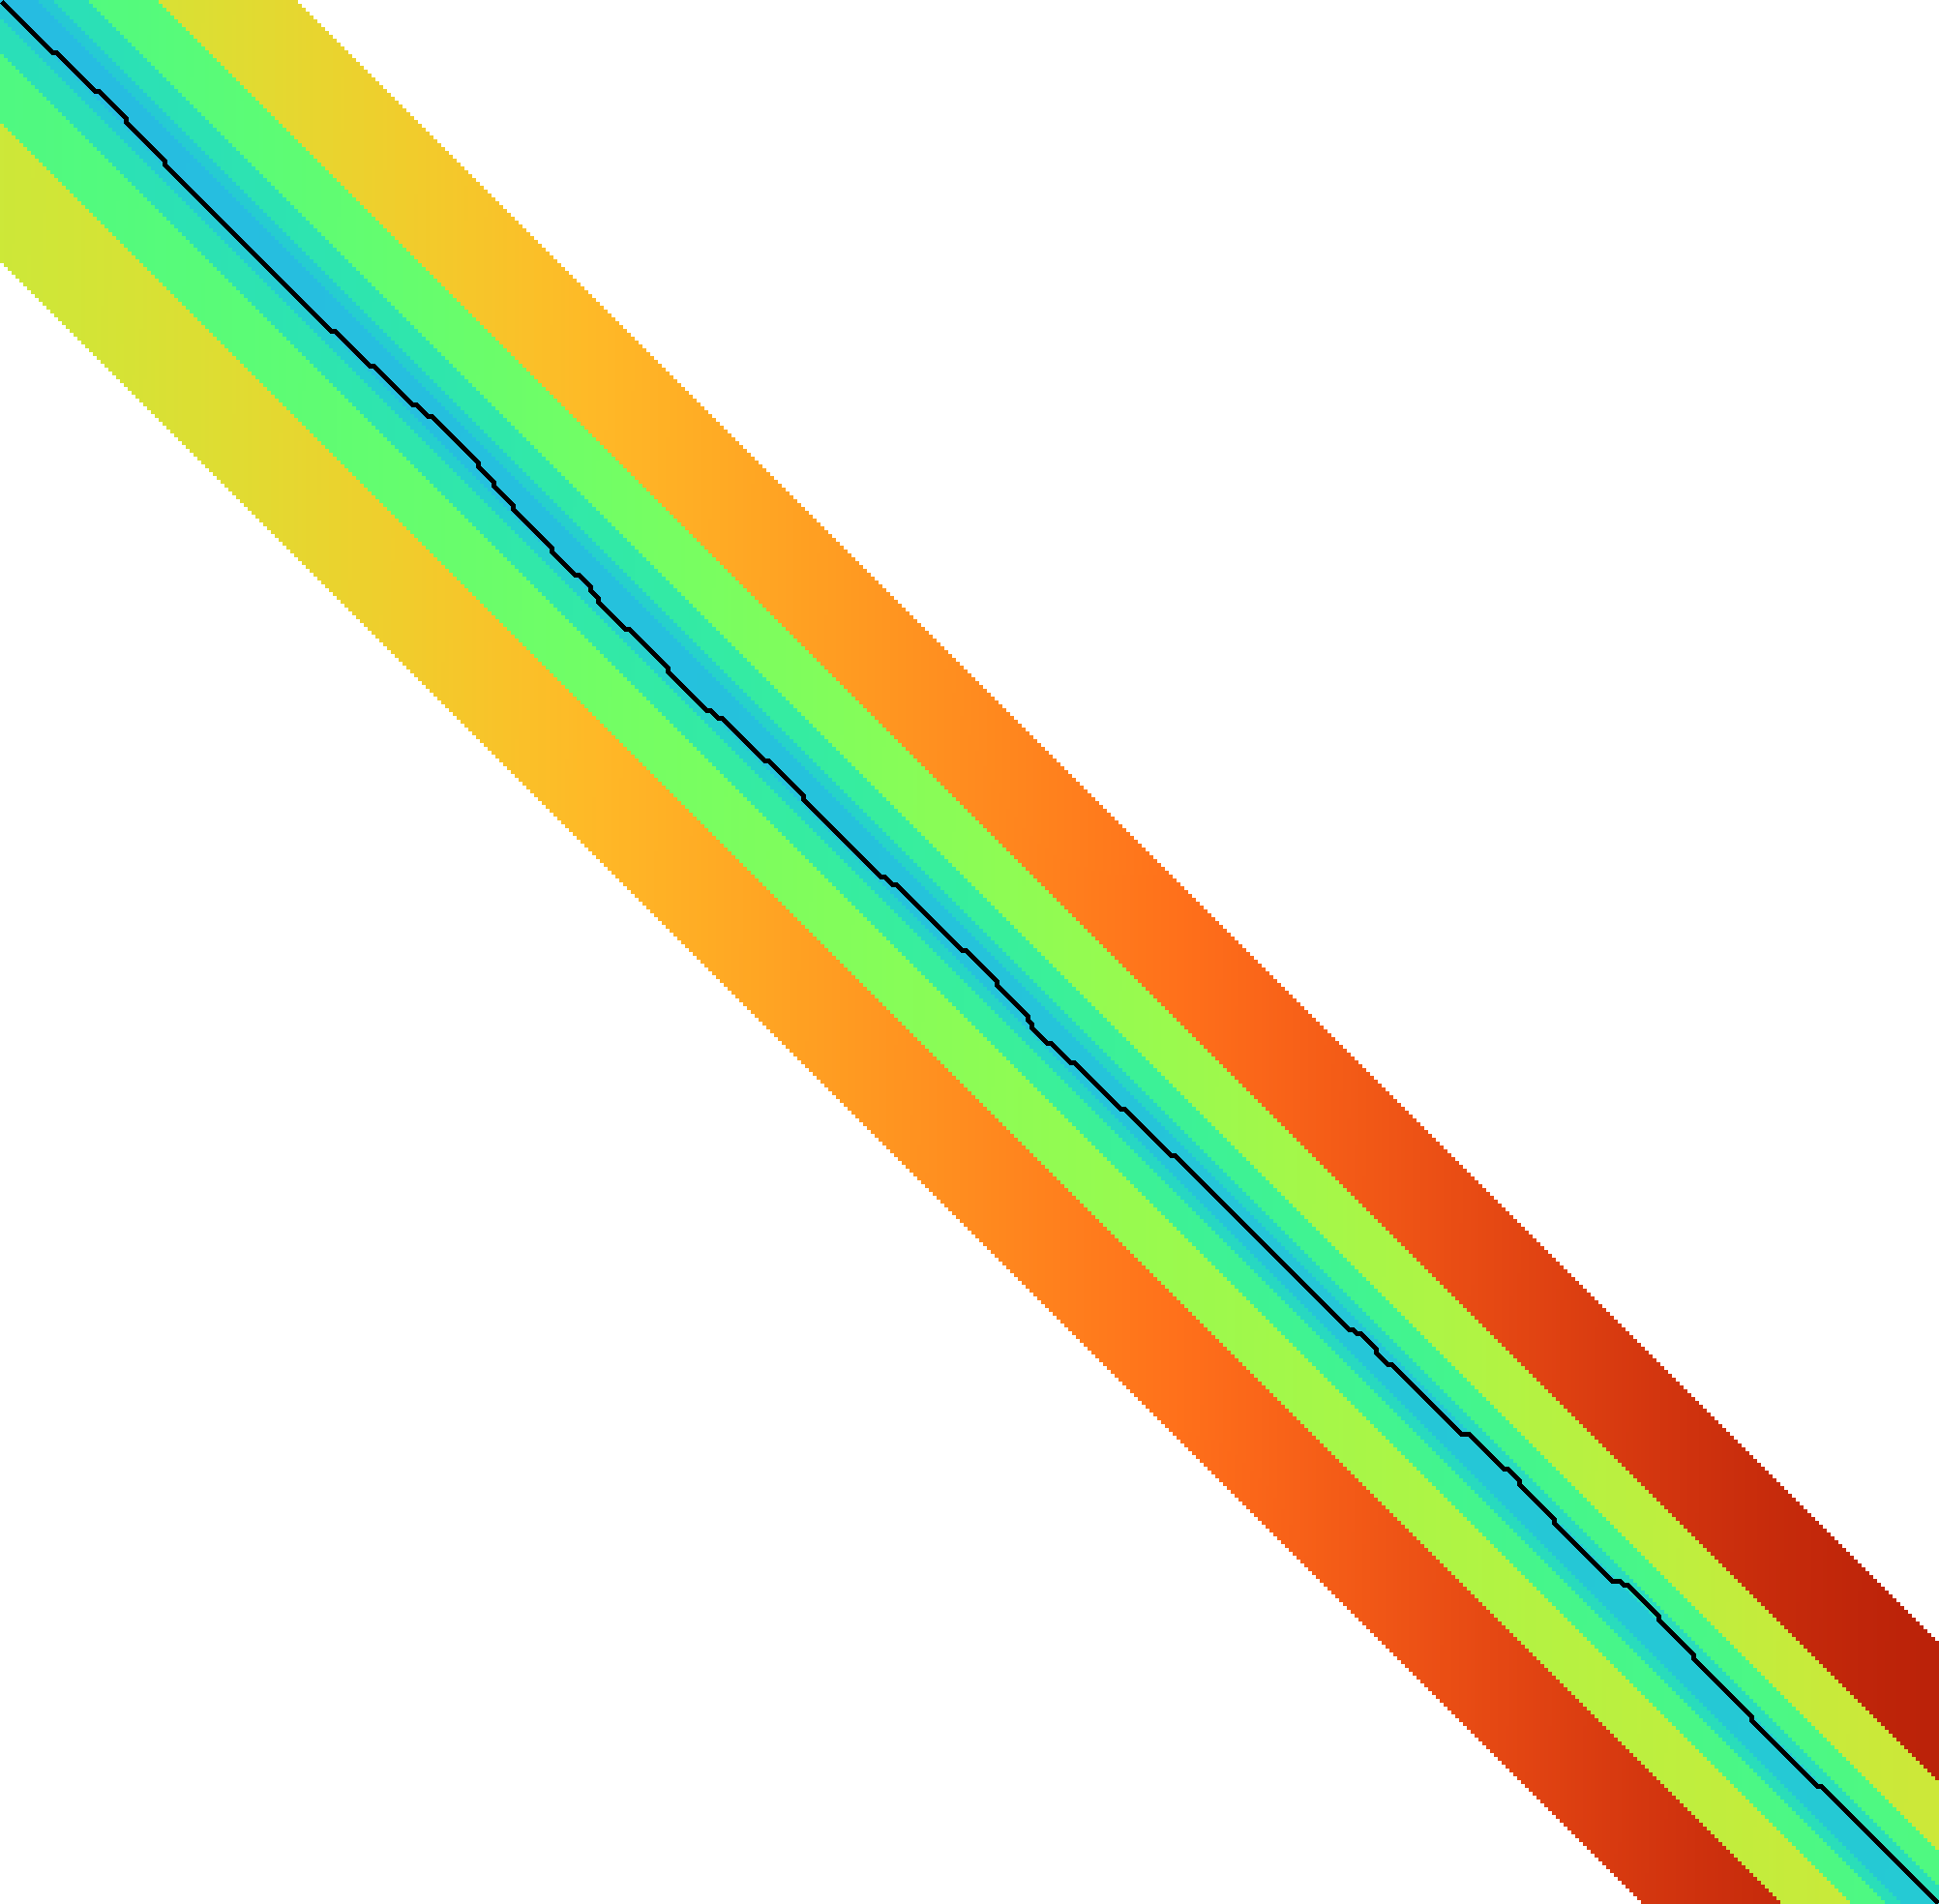
\includegraphics[width=0.33\linewidth]{imgs/intro/1_ukkonen.png}\label{fig1-band}}
    \hspace{-8em}
    \hfill
    \subfloat[\\\dijkstra] {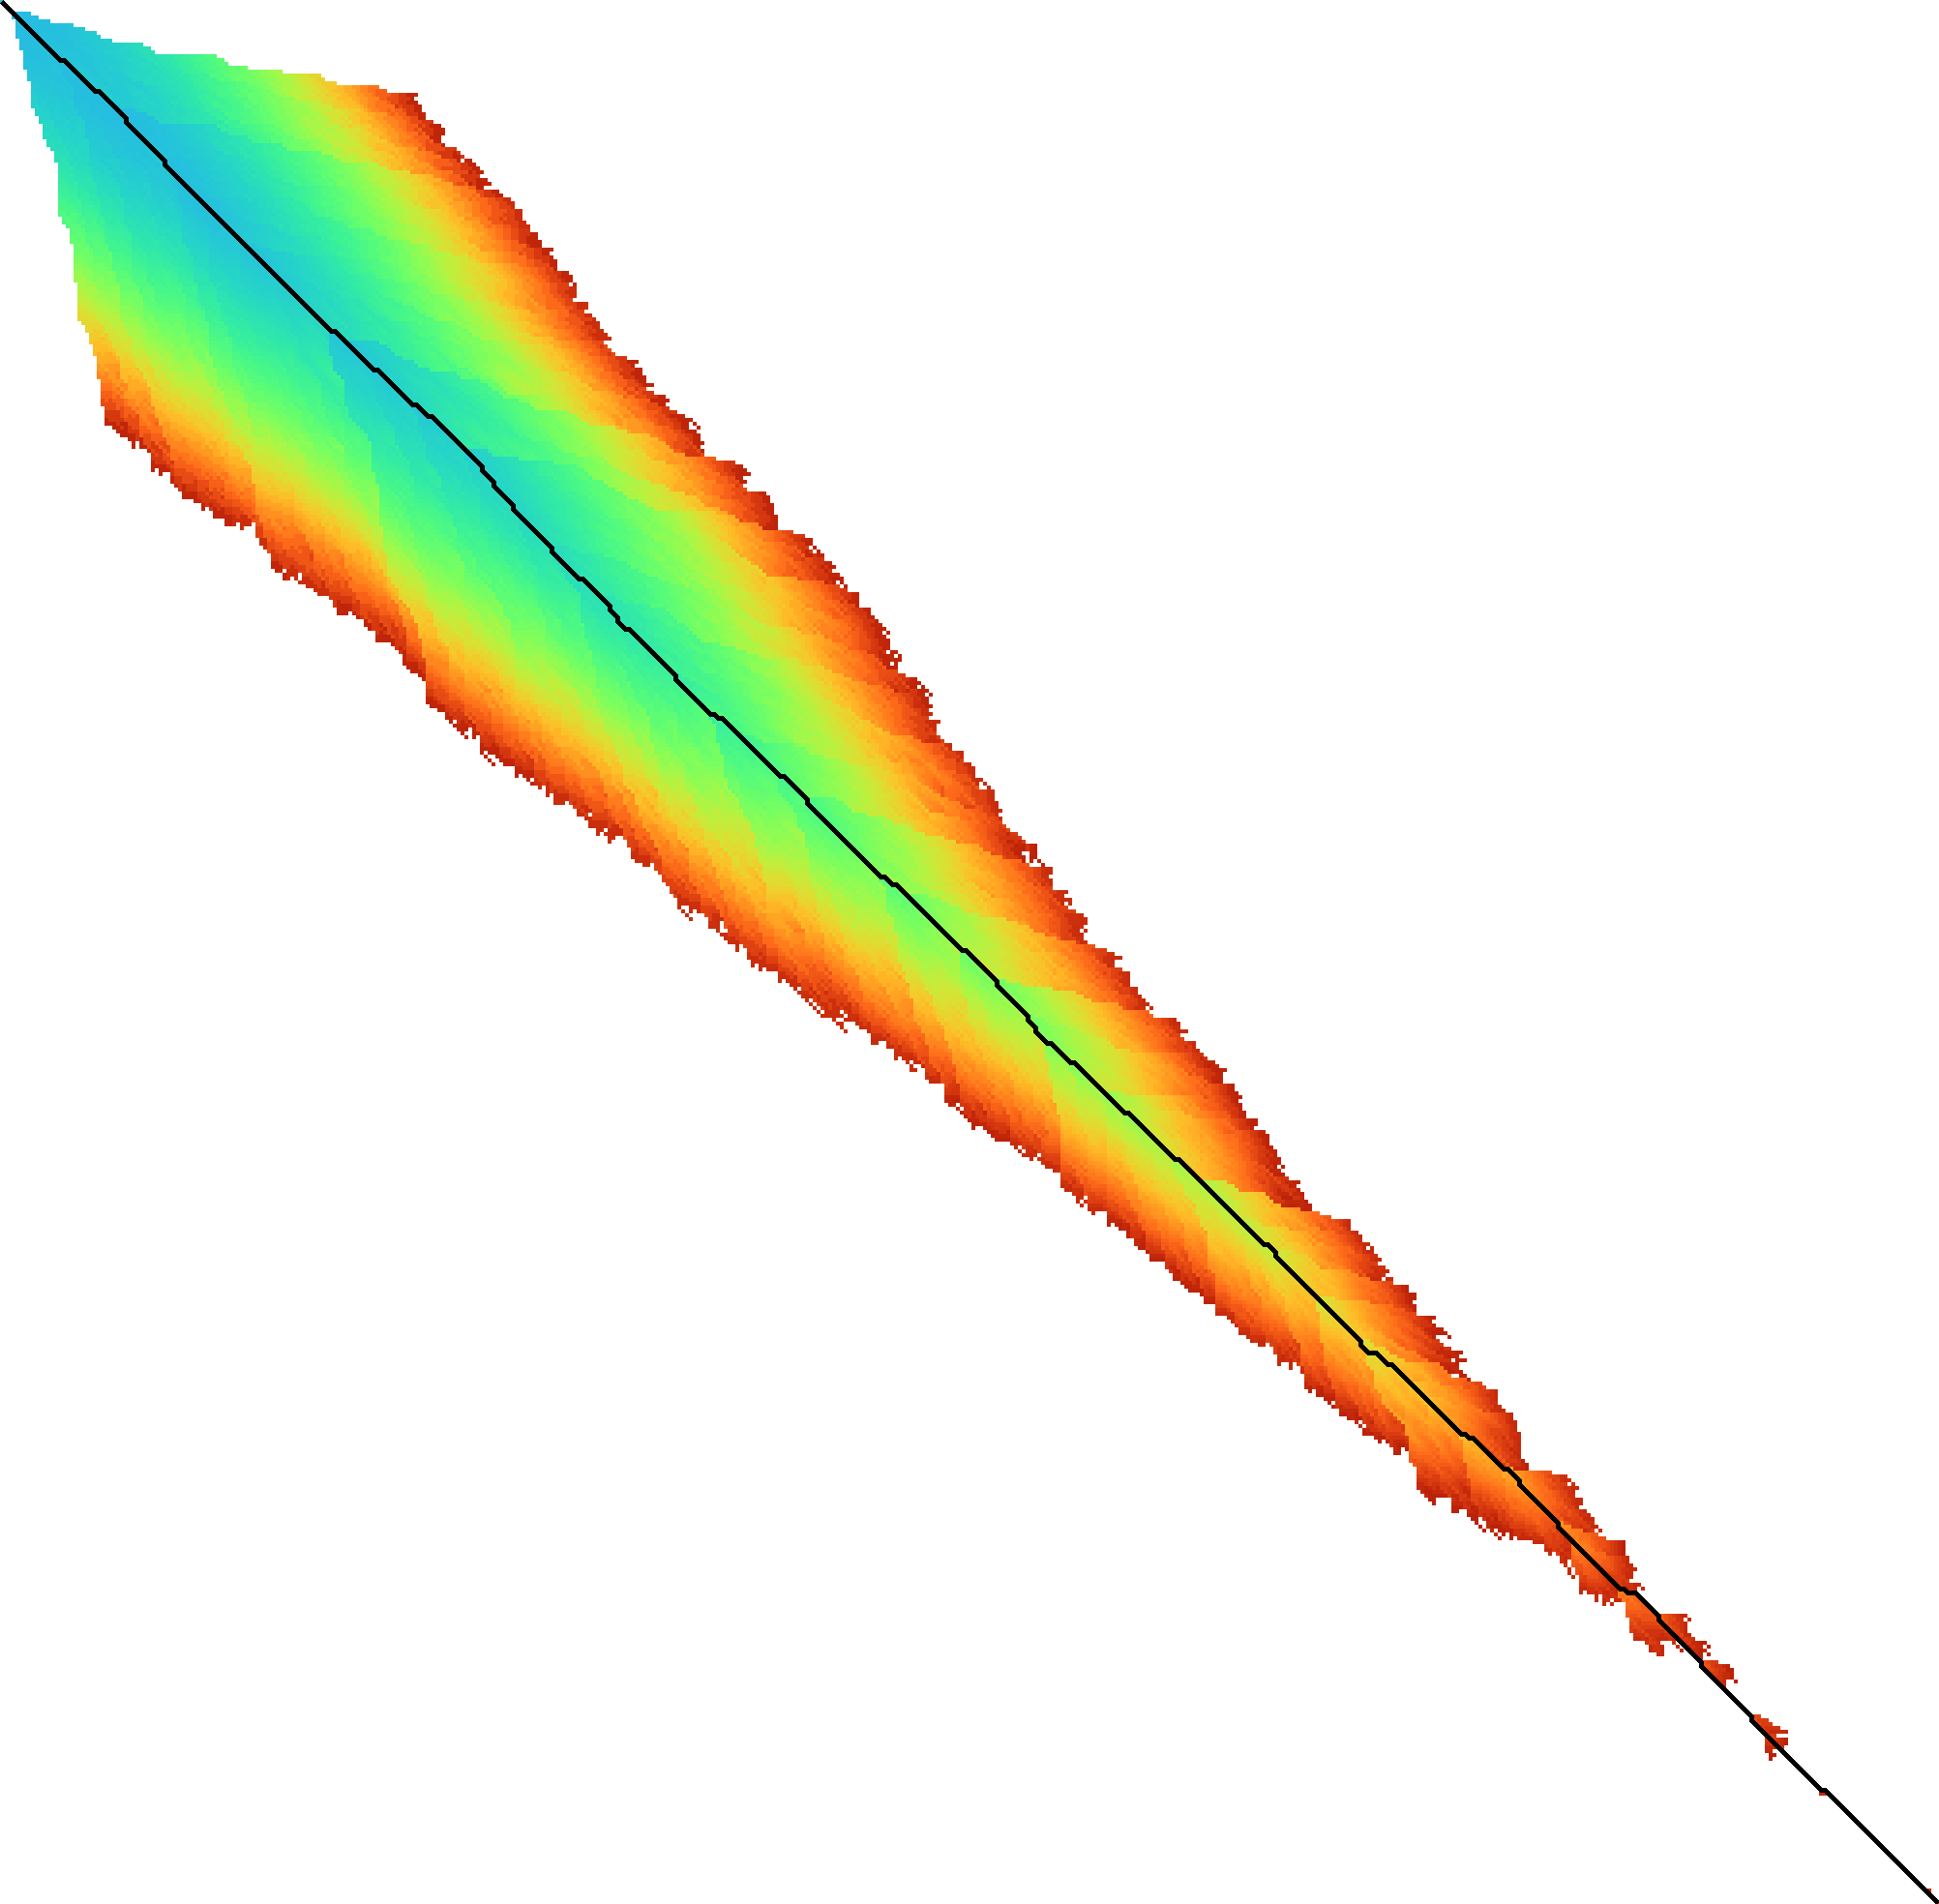
\includegraphics[width=0.33\linewidth]{imgs/intro/2_dijkstra.png}\label{fig1-dij}}
    \hspace{-8em}
    \hfill
    \subfloat[\\DT\\(\oldwfa)]{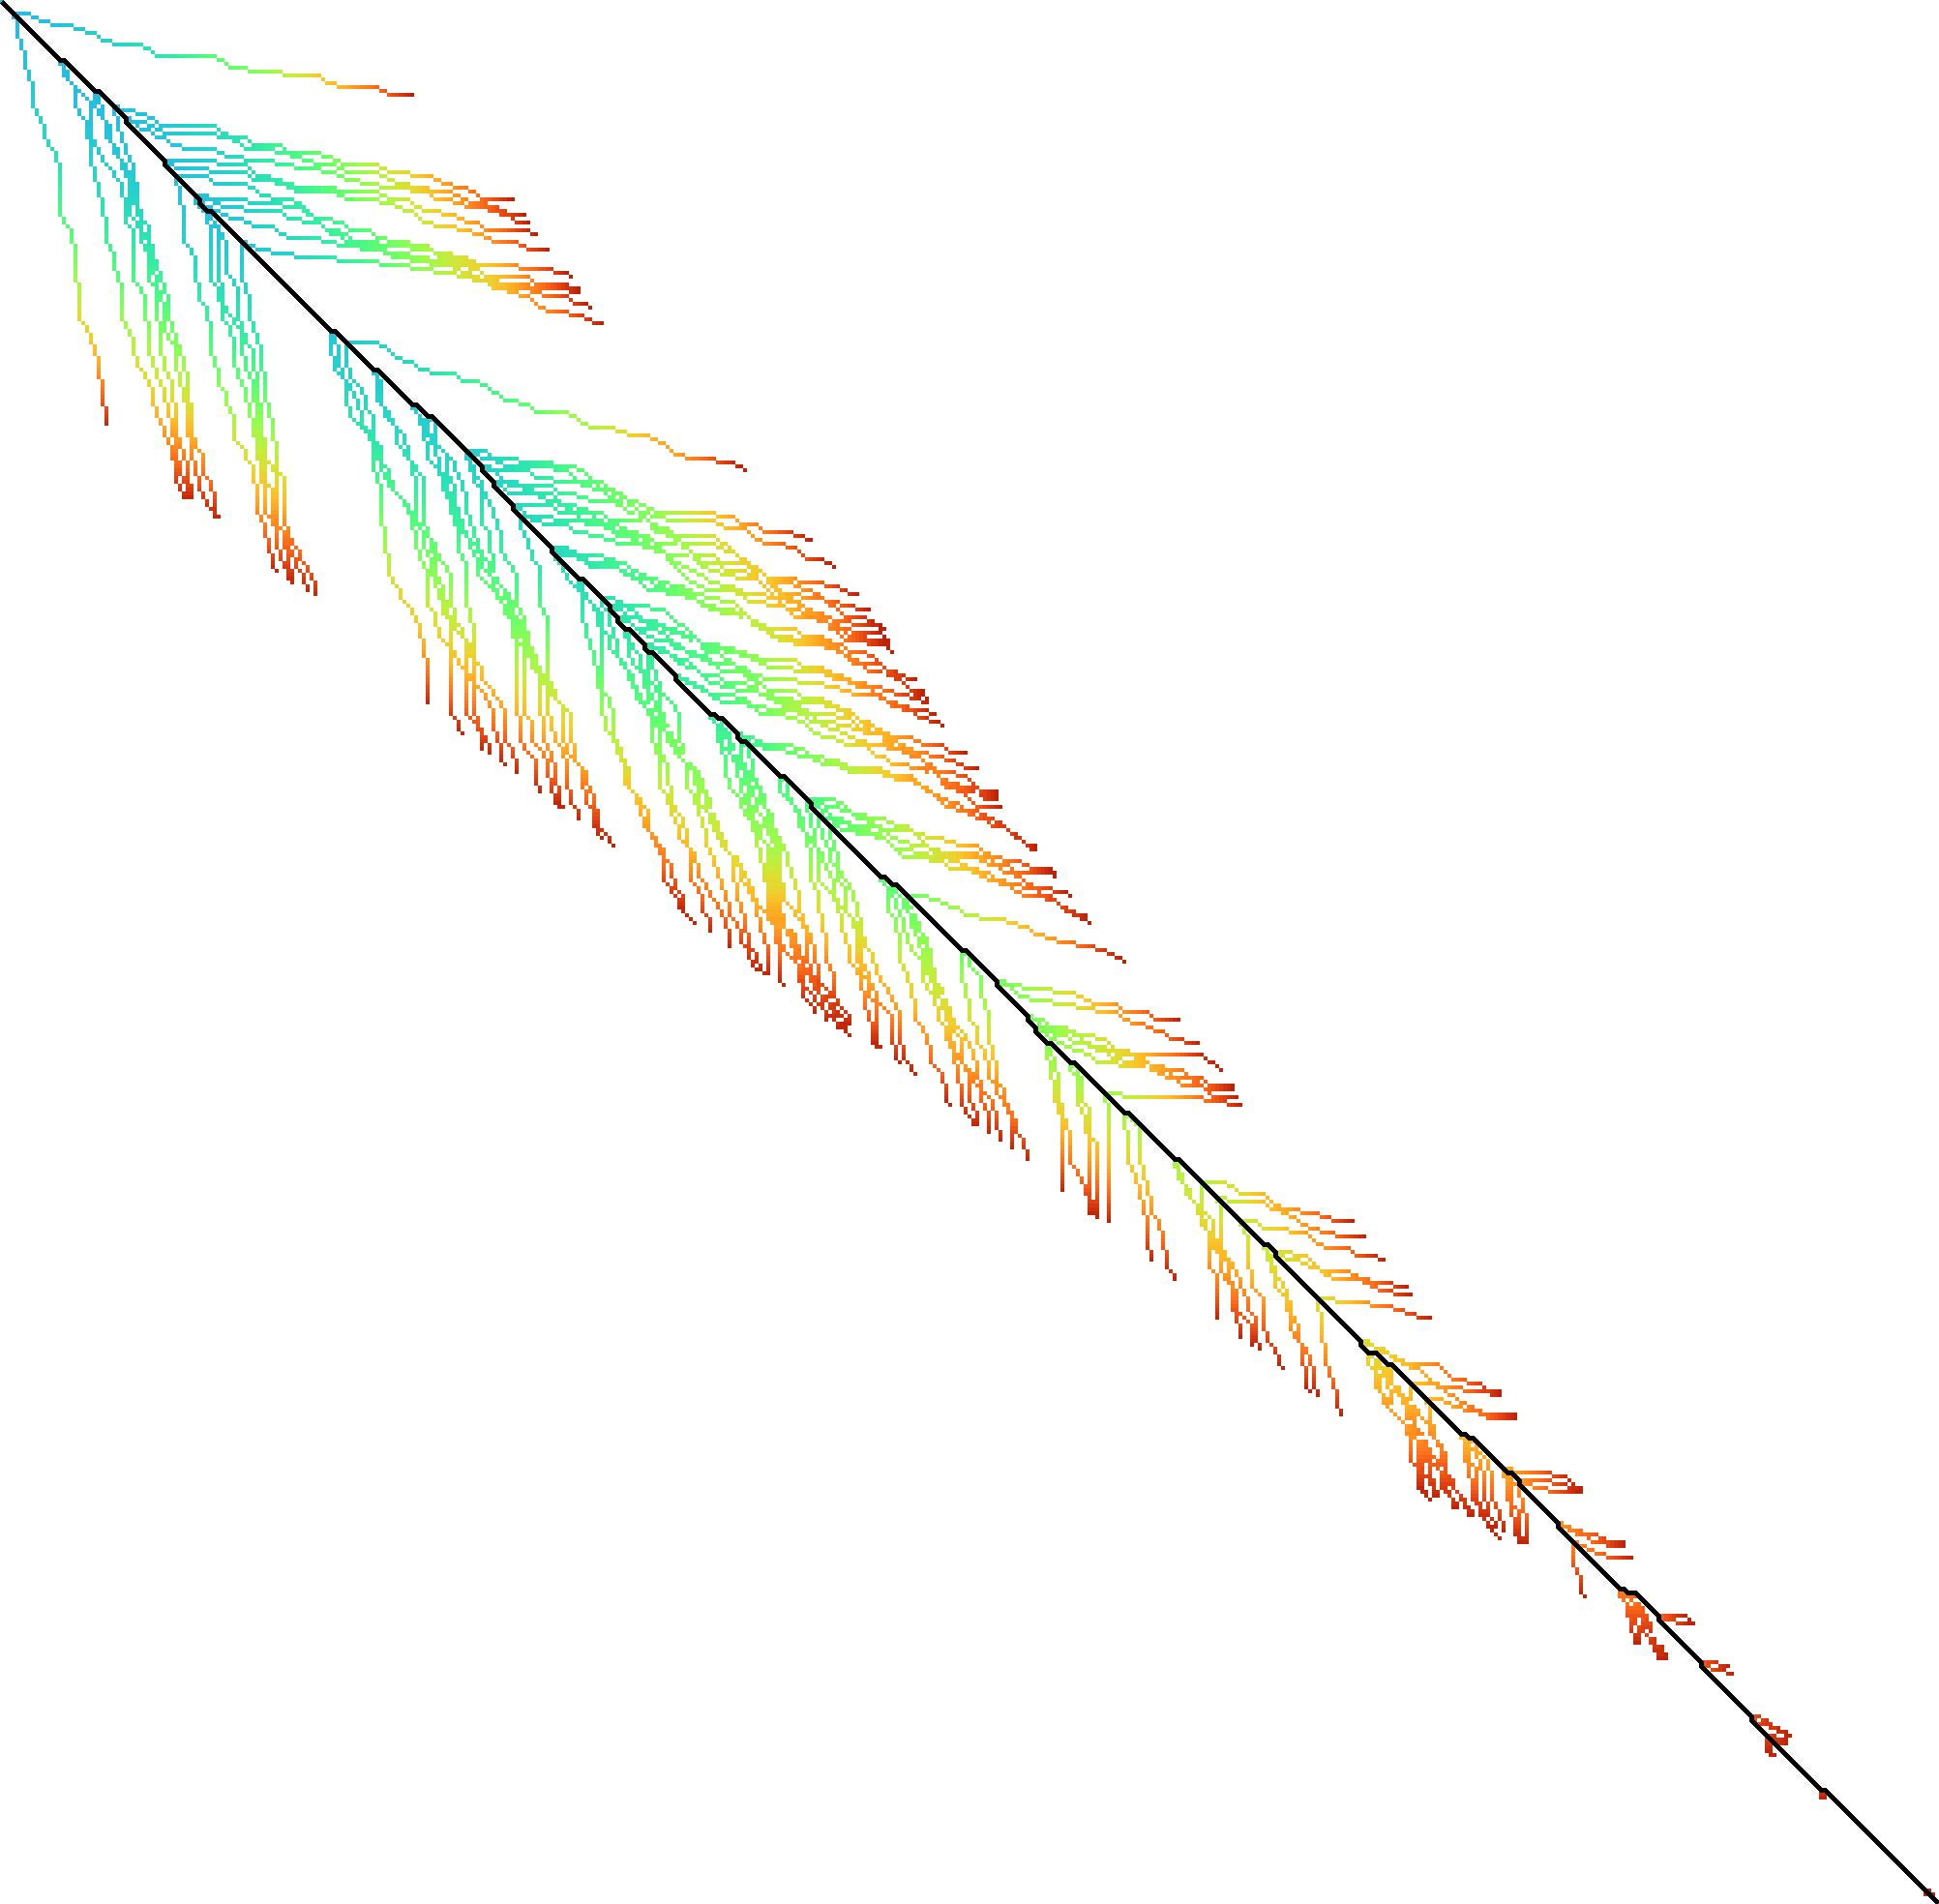
\includegraphics[width=0.33\linewidth]{imgs/intro/3_diagonal-transition.png}\label{fig1-wfa}}
    \hspace{-8em}
    \hfill
    \subfloat[\\DT+D\&C\\(\wfa)]{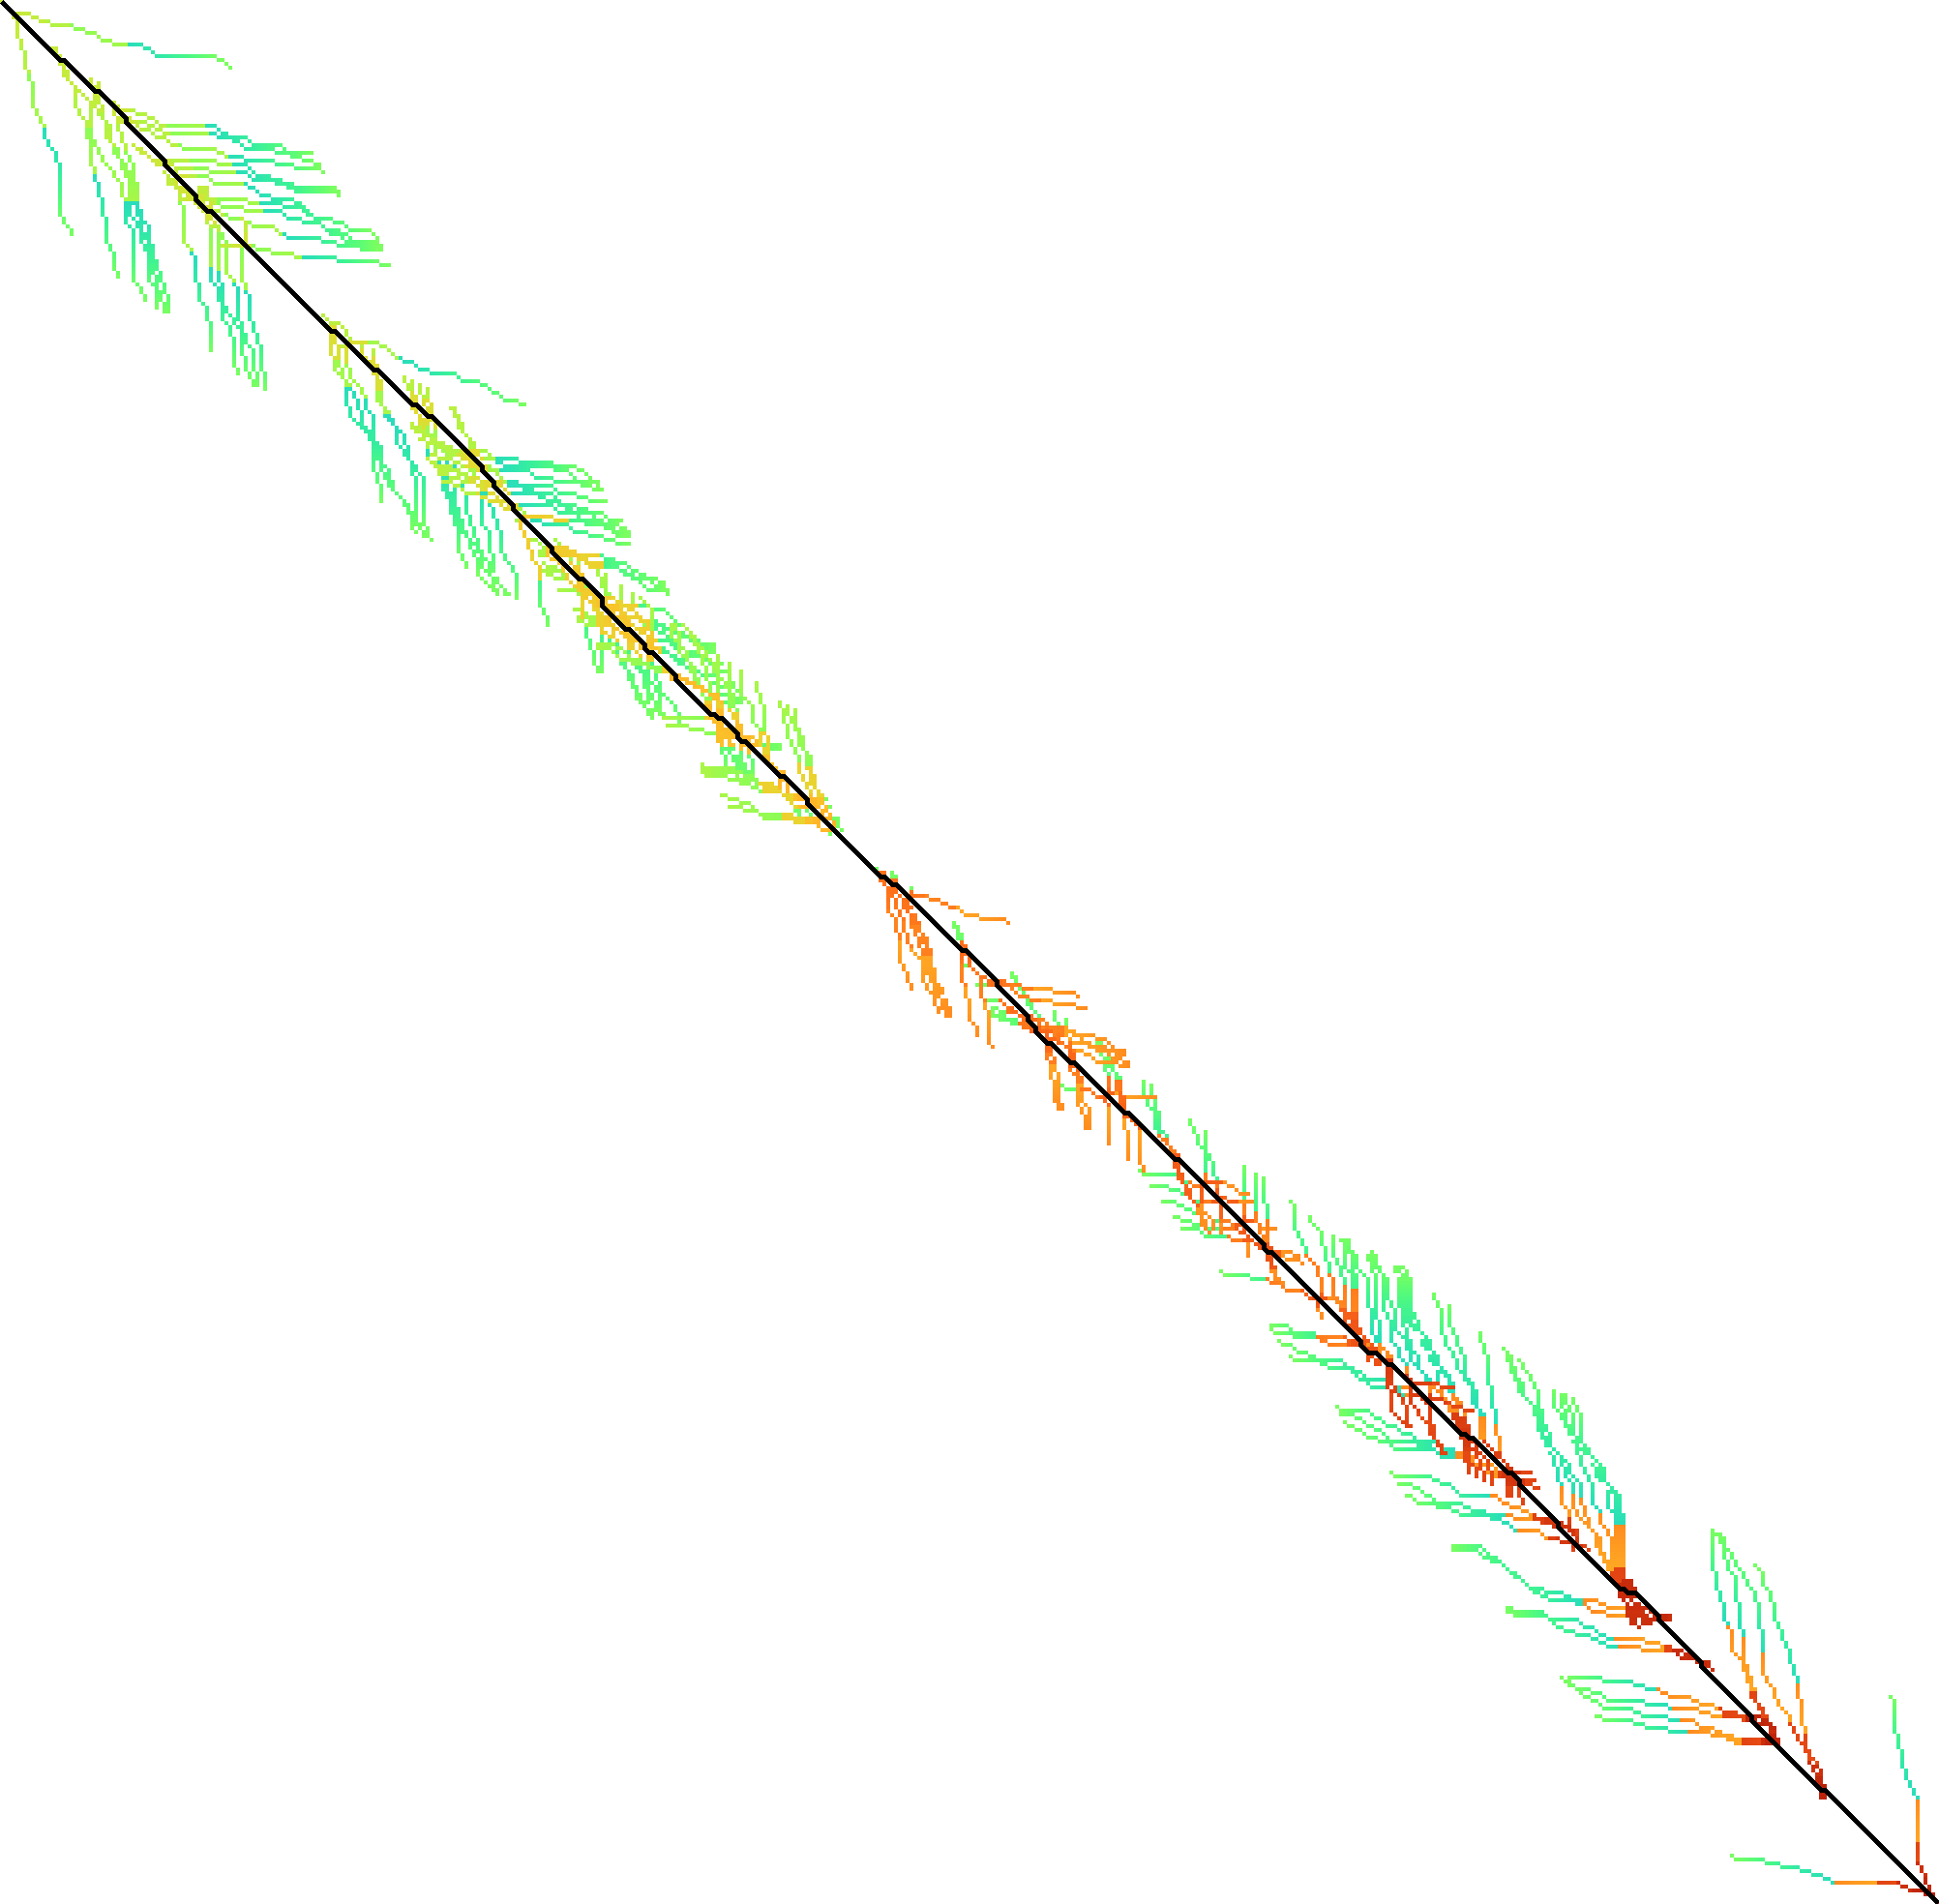
\includegraphics[width=0.33\linewidth]{imgs/intro/4_dt-divide-and-conquer.png}\label{fig1-biwfa}}
    \hspace{-8em}
    \hfill
    \subfloat[\\\textbf{This work}\\\textbf{(\astarpa)}]{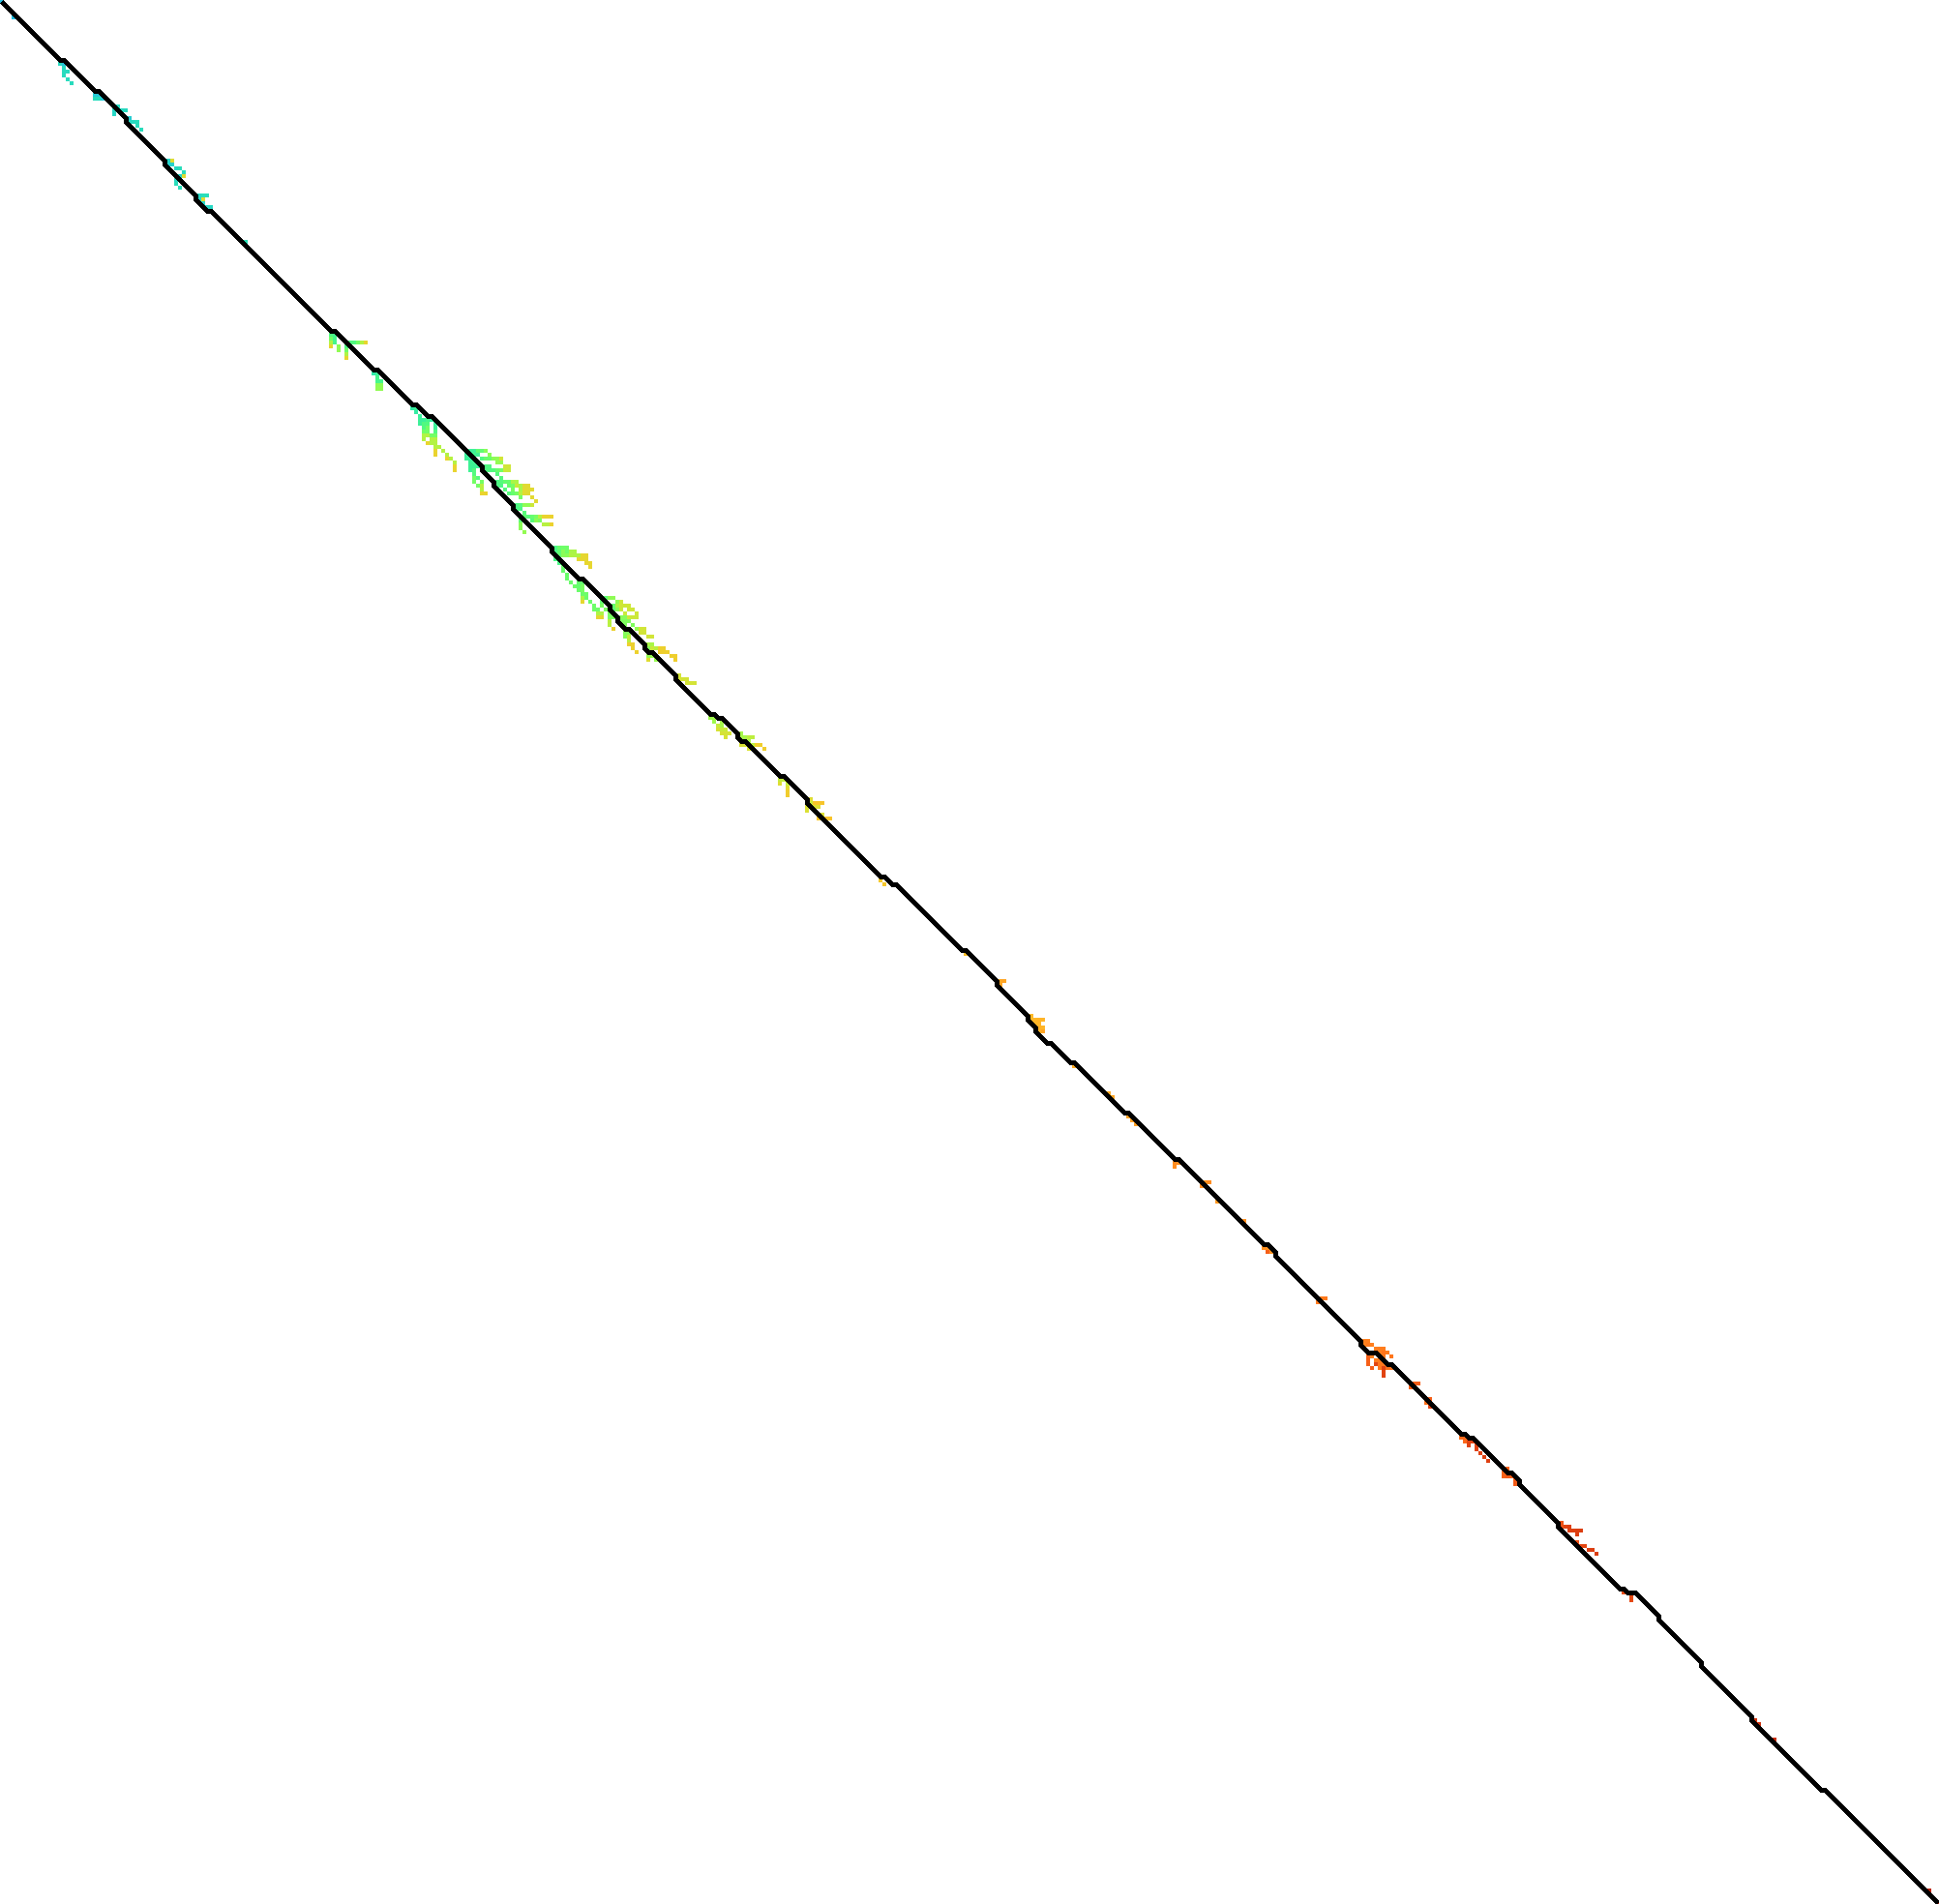
\includegraphics[width=0.33\linewidth]{imgs/intro/5_astarpa.png}\label{fig1-astar}}
    \caption[Computed states per global alignment algorithm.]{%
      \textbf{Computed states per algorithm.} Various optimal alignment
algorithms and their implementation are demonstrated on synthetic data (length
$n{=}500\bp$, divergence $d{=}16\%$). The colour indicates the order of
computation from blue to red. \protect\subref{fig1-band} Band-doubling (\edlib), \protect\subref{fig1-dij}
\dijkstra, \protect\subref{fig1-wfa} Diagonal transition/DT (\oldwfa), \protect\subref{fig1-biwfa} DT with
divide-and-conquer/D\&C (\wfa), \protect\subref{fig1-astar} \astarpa with \gch (\GCH), match
pruning, and DT (seed length $k{=}5$ and exact matches).}
    \label{fig:intro}
\end{figure}
